\documentclass[a4paper]{article}
\usepackage{praktikum}
\begin{document}
	
%%
%% Bitte das Deckblatt nicht verändern


\thispagestyle{empty}
\begin{center}

    {\large {\bf   BAI3-GKA WiSe2§ \\ Graphentheoretische Konzepte und Algorithmen \\[5mm]} }
    
{\huge Praktikumsaufgabe-Template  \\[5mm] Deckblatt}\\

\end{center}

				\begin{tabular}[t]{|r|l|}
				 \hline
%%%%				
%%%% Bitte  Ihren Namen und  Ihr Team und die Gruppe angeben
				GKA-Gruppe&                 \raisebox{-3mm}{\rule[8mm]{100mm}{0mm} }\\ \hline    
				Team &                                                        \\ \hline			
				& \textit{Iryna Trygub }               \\ \hline    
				& \textit{Ansgar Deuschel }               \\ \hline			
				& \textit{Kristoffer Schaaf }             \\ \hline  			
				\multicolumn{2}{c}{}\\  			
				\multicolumn{2}{l}{Bearbeitete Themen in Stichpunkten:}\\			
				\multicolumn{2}{c}{}\\  \hline
				Iryna Trygub &              \\ \hline    
				Ansgar Deuschel &                \\ \hline			
				Kristoffer Schaaf & Ops            \\ \hline 		
				\multicolumn{2}{c}{}\\  			
				\multicolumn{2}{l}{Geschätzte Arbeitszeiten in Stunden:}\\			
				\multicolumn{2}{c}{}\\  \hline
				Iryna Trygub &               \\ \hline    
				Ansgar Deuschel &                \\ \hline			
				Kristoffer Schaaf &               \\ \hline 			
				\end{tabular}
~\\[4mm]
		
		
\vfill


\newpage

\tableofcontents

\newpage

\section{Einleitung}

Der Kruskal-Algorithmus ist ein Greedy-Algorithmus, der verwendet wird, um den minimalen Spannbaum eines Graphen zu finden. Der Algorithmus funktioniert in mehreren Schritten:

\begin{enumerate} \label{Einleitung}
    \item Zuerst werden alle Kanten des Graphen nach ihrem Gewicht sortiert. Die Kante mit dem kleinsten Gewicht wird zuerst betrachtet. 

    \item Für jeden Knoten wird eine neue Teilmenge erstellt
    
    \item Für jede Kante (v1, v2) aus E, beginnend mit der kleinsten Gewichtskante:
    
        \begin{enumerate}
            \item Überprüfe, ob v1 und v2 in verschiedenen Teilmengen liegen. Wenn ja, füge die Kante dem minimalen Spannbaum hinzu und vereinige die beiden Teilmengen.
            \item Wenn v1 und v2 bereits in derselben Teilmenge sind, gehe zur nächsten Kante.
        \end{enumerate}
    
     \item Der Prozess wird fortgesetzt, bis alle Knoten im neuen Graphen verbunden sind oder alle Kanten betrachtet wurden. Wenn alle Knoten verbunden sind, stoppt der Algorithmus. Wenn noch Kanten übrig sind, werden sie ignoriert, da sie einen Kreis im Graphen verursachen würden.
\end{enumerate}

Der Kruskal-Algorithmus ist besonders nützlich in der Operations Research, insbesondere wenn es darum geht, die kostengünstigste Verbindung zwischen verschiedenen Stationen zu finden, beispielsweise beim Ausbau eines Schienennetzes\footnote{https://www.bwl-lexikon.de/wiki/kruskal-algorithmus/}. \\

\section{Laufzeit}

Die Laufzeit des Algorithmus hängt stark von Schritt 1 und 2 ab. Im Allgemeinen kann jeder Sortieralgorithmus verwendet werden, um die Kanten des Graphen zu sortieren. Unter Verwendung der Prioritätswarteschlange als Datenstruktur in Schritt 1 und 2 ist das Finden und Entfernen der kleinsten Kante in $O(log(n))$ Schritten möglich\footnote{https://docs.oracle.com/javase/7/docs/api/java/util/PriorityQueue.html}.

\section{Dokumentation der Implementierung}

\subsection{Disjoint Set}

Die Bibliothek Graphstream bietet eine eigene Implementierung des DisjointSet. Aufgabe hiervon ist es, die verschiedenen Teilmengen so zu verwalten, dass diese disjunkt zueinander sind. Wie in Anhang B2 beschrieben\cite{KN2012} werden drei verschiedene Operation für die Verwaltung der Teilmengen benötigt. Aufgrund einer fehlenden Operation in der Graphstream Implementierung und der fehlenden Erweiterbarkeit bedingt durch die Scopes der implementierten Operationen, haben wir uns dazu entschieden unser eigenes Disjoint Set zu implementieren. Dieses hat nach wie vor die drei benötigten Operationen, ist aber zustandslos und bietet somit nur statische Methoden.

\begin{itemize}
    \item \textit{makeSet($HashSet\langle Node\rangle$)} oder \textit{makeSet($HashSet\langle MultiGraph\rangle$)} \\Hierbei wird ein neues Set erstellt. Dieses hat den Typen HashSet und enthält weitere Teilmengen von Knoten. Auch diese werden in HashSets gespeichert. Final hat das DisjointSet also den Typen $HashSet\langle HashSet\langle Node\rangle \rangle$. \\Dieser Operation ein Set von Nodes übergeben werden, welches nach Operationsaufruf das einzige Element des Disjoint Sets wäre. Das entspräche der Vorgabe. Um aber direkt bei Initialisierung des DisjointSets die Teilmengen für jeden Knoten zu erstellen, gibt es eine Überschreibung der ersten Methodensignatur. In dieser wird ein Graph übergeben und ein initialisertes DisjointSet mit einer Teilmenge pro Knoten wird zurückgegeben. 
    \item \textit{union($HashSet\langle Node\rangle$, $HashSet\langle Node\rangle$, $HashSet\langle HashSet\langle Node\rangle \rangle$)} \\In dieser Funktion werden zwei Teilmengen konkateniert und dem DisjointSet hinzugefügt. Die ursprünglichen Teilmengen werden anschließend aus dem DisjointSet entfernt. Da das DisjointSet zustandslos ist, muss die Operation zusätzlich das bisherige DisjointSet mit als Parameter übergeben bekommen. In diesem Punkt unterscheidet sich unsere Implementierung von der Vorgabe.
    \item \textit{find-set($HashSet\langle HashSet\langle Node\rangle \rangle$, Node)} \\Diese Operation sucht die Teilmenge in dem DisjointSet, welche den übergebenen Knoten enthält. Auch hier muss aufgrund der Zustandslosigkeit das DisjointSet mit als Parameter übergeben werden.
\end{itemize}

\subsubsection{Laufzeit DisjointSet}

Die Methoden add(), remove() und contains() des HashSets haben eine Komplexität von $O(1)$\footnote{https://www.baeldung.com/java-collections-complexity}. Somit hat make-set eine Komplexität von $O(1)$, union $O(1)$ und find-set $O(n)$.

\subsection{Rückgabewert Kruskal}

Der Rückgabewert der Kruskal Methode createMinimalSpanningForrest(Multigraph graph) ist ein neu erzeugtes KruskalResult Objekt. In diesem ist der Spannwald als Graph und als Set aus Kanten enthalten. Zusätzlich ist die gesamte Größe der Kantengewichte gespeichert. Zur Erzeugung des Spannwaldgraphen wird die Hilfsfunktion createSpanningForrestGraph(Multigraph graph, $HashSet\langle Edge\rangle$ minimalSpanningTree) genutzt. In dieser wird über alle Kanten des minimalen Spannwaldes iteriert und ein entsprechender Graph zusammengebaut. 

\subsubsection{Alleinstehende Knoten im Spannwald}

Anhand Punkt 1 in der Einleitung\ref{Einleitung} wird ersichtlich, dass alleinstehende Knoten - also Knoten ohne Kanten - durch die fehlenden Kanten nicht weiter beachtet werden. Hierfür wurde eine neue Funktion eingeführt, welche alle betroffenen Knoten zu Beginn in einem Set speichert und diese dann dem Graph hinzufügt, welcher den Spannwald final darstellt. 

\subsection{Die Main Methode}

In der Main Methode wird der Kruskal Algorithmus auf einen zufällig generierten Graphen angewendet. Die Größe des Graphen muss hierfür hart gecoded werden. Damit nach Ausführung der Main Methode der zufällig generierte Graph betrachtet werden kann, wird dieser über den GraphFileWriter des letzten Praktikums in eine Datei im Pfad \textit{src/main/resources/graphs} abgelegt. Ein Ausschnitt aus einer solchen Datei könnte so aussehen:

\begin{lstlisting}[frame = trBL]
#undirected:Graph;
node196-node122(edge63)::1;
node63-node52(edge1075)::1;
\end{lstlisting}

Die Summe aller Kantengewichte aus dem minimalen Spannwald ist in dem KruskalResult Objekt enthalten. Dieses wird in der Konsole ausgegeben, bevor der finale minimale Spannwald visualisiert wird. Zusätzlich steht in der Konsole, wie viele Knoten und Kanten der erzeugte Graph enthalten hat.

\newpage

\section{Tests}

\subsection{Fest definierte Testgraphen}

Getestet wird zum einen mit verschiedenen fest definierten Testgraphen. Diese entsprechen bestimmten Vorgaben und sollten alle relevanten Edge Cases abdecken.\\

Der erste zu testende Graph ist der Testgraph aus der letzten Praktikumsaufgabe\ref{fig:beispielgraph_4}. Soweit gibt es in diesem Graphen keine Edge Cases. Der Test dient lediglich einmal den Happy Path zu testen.

\begin{figure}[htbp]
	\centering
		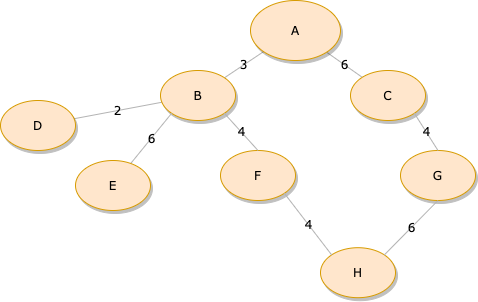
\includegraphics[width=0.50\textwidth]{Latex/Figs/Beispielgraph_4.png}		
	\caption{Ein zusammenhängender Graph}
	\label{fig:beispielgraph_4}
\end{figure}

Der zweite Graph besteht aus zwei nicht zusammenhängenden Teilgraphen\ref{fig:beispielgraph_2}. Da in dieser Aufgabe nicht nur ein Spannbaum sondern ein Spannwald erstellt werden soll. Muss der Algorithmus entsprechend auch auf einem nicht zusammenhängendem Teilgraphen getestet werden. Dass die beiden Graphen die gleiche Anzahl an Knoten und an Kanten mit den gleichen Gewichten hat, ist nicht weiter relevant.

\begin{figure}[htbp]
	\centering
		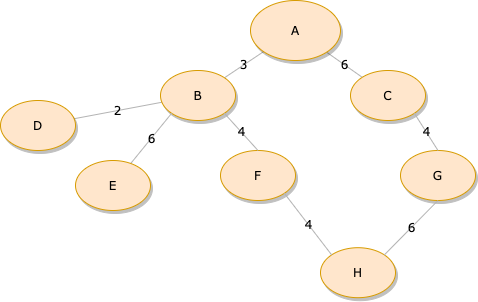
\includegraphics[width=0.60\textwidth]{Latex/Figs/Beispielgraph_2.png}		
	\caption{Zwei nicht zusammenhängende Graphen}
	\label{fig:beispielgraph_2}
\end{figure}

Ein spannender Fall ist das Betrachtet eines einzelnen Knotens als Graphen\ref{fig:beispielgraph_3}, wenn dieser keine Kanten hat. Durch die Implementation werden in den meisten Fällen nur Knoten beachtet, welche auch Kanten haben, da diese ansonsten nicht in der Prioritätswarteschlange referenziert werden. Die Definition eines minimalen Spannbaums lautet allerdings: Ein minimaler Spannbaum ist ein Baum, der alle Knoten eines Graphen verbindet und dabei die minimale Summe der Kantengewichte hat\footnote{https://en.wikipedia.org/wiki/Minimum\_spanning\_tree}. In diesem speziellen Fall ist der Graph selbst ein Baum und da es keine Kanten gibt, ist die Summe der Kantengewichte gleich Null. Daher ist der Graphen selbst der minimale Spannbaum.

\begin{figure}[htbp]
	\centering
		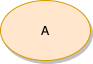
\includegraphics[width=0.1\textwidth]{Latex/Figs/Beispielgraph_3.png}		
	\caption{Graph mit einem einzelnen Knoten}
	\label{fig:beispielgraph_3}
\end{figure}

Der Vollständigkeit halber testen wir auch einen Graphen welcher aus zwei nicht zusammenhängenden Teilgraphen besteht\ref{fig:beispielgraph_1}. Der eine besteht aus einem Graphen ohne Edge Cases, der zweite ist ein einzelner Knoten ohne Kanten. 

\begin{figure}[htbp]
	\centering
		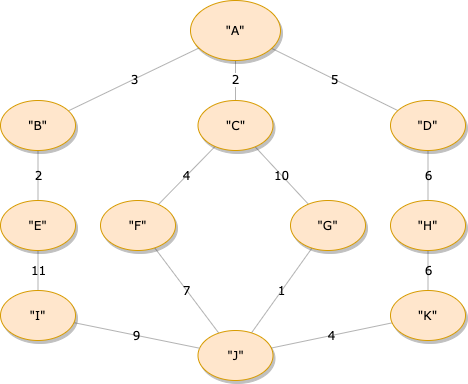
\includegraphics[width=0.55\textwidth]{Latex/Figs/Beispielgraph_1.png}		
	\caption{Zwei nicht zusammenhängende Graphen, einer mit einem einzelnen Knoten}
	\label{fig:beispielgraph_1}
\end{figure}

\subsection{Zufällig generierte Graphen}

Als Feedback vom letzten Praktikum haben wir mitgenommen, dass wir auch mit zufällig generierten Graphen testen sollen. Ein Problem hierbei ist offensichtlich wie das Ergebnis generisch getestet werden soll. Hierfür bietet sich der Kruskal Algorithmus der Graphstream Bibliothek an. Wie oben beschrieben gibt auch dieser einen Graphen zurück und kann somit verglichen werden.\\
Generiert werden unsere Graphen über den GraphGenerator. Dieser erwartet als Parameter die Anzahl an Knoten und Kanten, das maximale Gewicht der Kanten und ob diese gerichtet sein sollen. Der zurückgegebene Graph ist entweder vollständig ungerichtet oder vollständig gerichtet.

\subsubsection{Assertions}

Das Überschreiben der Equals Methode des Graphs von Graphstream erschien in unserem Fall zu aufwändig. Wir hätten hierfür bereits bestehenden Code stark refactoren müssen. Außerdem sind sowohl im Typen Kruskal als auch Prim nur die Felder \textit{graph} und \textit{treeEdges} gespeichert. \textit{graph} ist hierbei der unveränderte Originalgraph und \textit{treeEdges} ist eine Liste mit allen Kanten des minimalen Spannwaldes. Bei größeren Graphen besteht die Möglichkeit, dass unser Kruskal Algorithmus einen anderen minimalen Spannbaum findet als die GraphStream Algorithmen Kruskal oder Prim. Als mögliche Assertions für die Tests mit zufällig erzeugten Graphen kommt also nur das Vergleichen der aufsummierten Kantengewichte in Frage.\\
Damit die Tests aussagekräftig sind, haben wir die Kantengewichte in einem möglichst großen Bereich (1-100) zufällig generiert.

\subsubsection{Ergebnisse und Laufzeit der Tests}

\begin{table}[htbp]
    \centering
    \begin{tabular}{||l|l|l|l|l||}
    \hhline{|t:=====:t|}
    \textbf{Nr} & \textbf{Name} & \textbf{Knoten} & \textbf{Kanten} & \textbf{Dauer (min)} \\ \hhline{|-----|}
         1 & Kruskal FewerNodesThanEdges & 50000 & 450000 & 4,88 \\ \hhline{|-----|}
         2 & Prim FewerNodesThanEdges & 50000 & 450000 & 0,0065 \\ \hhline{|-----|}
         3 & Kruskal SameNodesThanEdges & 75000 & 75000 & 4,84 \\ \hhline{|-----|}
         4 & Prim SameNodesThanEdges & 75000 & 75000 & 0,0046 \\ \hhline{|-----|}
         5 & Kruskal MoreNodesThanEdges & 100000 & 50000 & 4,99 \\ \hhline{|-----|}
         6 & Prim MoreNodesThanEdges & 100000 & 50000 & 0,0043 \\ \hhline{|b:=====:b|}
    \end{tabular}
    \caption{Open List}
    \label{laufzeit}
\end{table}

In der obigen Tabelle \ref{laufzeit} ist die Laufzeit unseres Kruskalalgorithmus im Vergleich zu dem Primalgorithmus von graphstream dargestellt.\\
Auffällig ist, dass eine Steigerung der Kantenanzahl zu einem geringeren Anstieg der Laufzeit führt, als bei einem gleichzahligen Anwachsen der Knotenanzahl. 
Da der Algorithmus über die Kanten iteriert, können wir uns dieses Phänomen nicht erklären. Zum Finden der kantenlosen Knoten iterieren wir auch über die Knoten, dies jedoch mit einer Zeitkomplexität von O(n) und über Streams.\\
Außerdem ist zu beachten, dass der Primalgorithmus deutlich schneller läuft.

\bibliographystyle{alpha}
\bibliography{mybib}

\end{document}